\documentclass[a4paper, 14pt]{article}

\usepackage[english, russian]{babel}
\usepackage[T2A]{fontenc}
\usepackage[utf8]{inputenc}
\usepackage{indentfirst}





\frenchspacing   
\usepackage{amsmath,amsfonts,amssymb,amsthm,mathtools}
\usepackage{graphicx} % for reflect boc
 % пакеты AMS
\usepackage[hidelinks]{hyperref}

\usepackage{icomma}                                    % "Умная" запятая
\usepackage{NiceMatrix}

\usepackage{physics}
\usepackage{slashed}
\usepackage{tikz}
\usepackage{geometry}
\geometry{top=25mm}
\geometry{bottom=30mm}
\geometry{left=20mm}
\geometry{right=20mm}

\linespread{1}

%Колонтитулы
\usepackage{titleps}
\newpagestyle{main}{
	\setheadrule{0.4pt}
	\setfootrule{0.4pt}
	\setfoot{}{\thepage}{}
}
\pagestyle{main}
\newcommand{\deriv}[2]{\frac{\partial #1}{\partial #2}}
\newcommand{\cderiv}[2]{\cfrac{\partial #1}{\partial #2}}
\newcommand*{\Eval}[3]{\left.#1\right\rvert_{#2}^{#3}}

\newcommand{\fderiv}[2]{\frac{d #1}{d #2}}
\newcommand{\tderiv}[1]{\frac{d #1}{d t}}

\newcommand{\cfderiv}[2]{\cfrac{d #1}{d #2}}
\newcommand{\ctderiv}[1]{\cfrac{d #1}{d t}}

\newcommand{\sn}[2]{\ensuremath{{#1}\cdot 10^{#2}}}

\newcommand{\dxv}[1]{d^3 {#1}}
\newcommand{\dpv}[1]{\cfrac{d^3 {#1}}{(2\pi)^3}}

\newcommand{\lvec}[1]{\reflectbox{\ensuremath{\vec{\reflectbox{\ensuremath{#1}}}}}}
\begin{document}
	Факты о потенциале.
	\subsubsection{Обозначения}
	\begin{enumerate}
		\item $\varphi(r)$ --- безразмерный положительный потегнциал.
		\begin{itemize}
			\item $\varphi(r) > 0$
			\item $\varphi(r) = \cfrac{1}{r}, r \ge 1$
			\item $\varphi'(r) < 0$
			\item $\varphi''(r) + \cfrac{2}{r}\varphi'(r) = -\rho(r) < 0$
		\end{itemize}
		\item $e$ --- положительная энергия
		\item $l$ --- момент импульса
		\item $l_m(e)$ --- максимальный момент импульса при данной энергии, $r_m(e)$ --- точка достижения этого максимума.
		\begin{equation}
			l^2_m(e) = \max_r{r^2(\varphi(r)-e)}
			\label{eq:l_m_e}
		\end{equation}
		\item $x_l = \sqrt{1 - \cfrac{l^2}{l_m^2}}$
		\item $T(e,l)$ --- время траектории.
		\begin{equation*}
			T(e,l) = \int_{r_{-}}^{r_{+}}\frac{dx}{ \sqrt{\varphi(x) -e - \frac{l^{2}}{x^{2}}}}
		\end{equation*}
		\begin{itemize}
			\item $T(e,l) - \cfrac{\pi}{2e^{3/2}}$ --- ограниченная гладкая функция параметров $e, x_l l_m$.
		\end{itemize}
		\item $r_{\pm}$ --- корни уравнения $r^2\varphi(r)-er^2-l^2=0$
		\item $u = r^2$, $u_{\pm}$ --- корни уравнения  $u\varphi(u)-eu-l^2=0$
		\item $F(u) = u\varphi(u)$ --- монотонная, гладкая, выпуклая вниз функция.
		\item $u_{-} \downarrow e, \uparrow l^2$
		\item $u_{+} \downarrow e, \downarrow l^2$
	\end{enumerate}
	
	
	\subsubsection{$l_m(e)$}
	Для нахождения $l_m(e)$ находятся $r_{i-1},r_i, r_{i+1}$ --- точки, такие, что $r_i \ge r_{i\pm1}$, далее фунция $F(u)$ приближается параболой, после чего находятся $u, l_m$
	
	Заметим, что если $e>\cfrac{1}{2}$, то максимальный момент равен
	\begin{equation*}
		l^2_m(e) = \cfrac{1}{4e}
	\end{equation*}
	однако траектории, пересекающие границу небесного тело ($\exists t: r(t,e,l) < 1$) ограничиваются $l^2 \le 1 - e$
	
	
	
	
		\subsubsection{Траектории.}
	При расчете траектории, делаем замену
	\begin{equation}
		u = \cfrac{u_{-}+u_{+}}{2} - \cfrac{u_{+}-u_{-}}{2}cos(\theta)
		\label{eq:tr_in_func}
	\end{equation}
	\begin{equation*}
		\dot{\theta} = 2\sqrt{ \cfrac{u\varphi(u)-eu-l^2}{(u-u_{-})(u-u_{+})} } = 2\sqrt{S(u)}
	\end{equation*}
	
	\begin{enumerate}
		\item если $e > 1/2$, то будем линейно интерполировать $\theta(e,l,\tau)$ ($\tau = t/T(e,l)$) по параметрам $e, \sqrt{l^2_m(e) - l^2}$
		
		Однако при интегрировании по траектории методом монте-карло, мы можем взять приближенную траекторию $\widetilde{\theta}(t)$, тогда, так как для истинной траектории $F(\theta)dt = d\theta$, то для приближенной таектории $\widetilde{F}(t')dt' = d\widetilde{\theta}$, т.е. 
		\begin{equation*}
			dt = \cfrac{\widetilde{F}(t')}{F(\theta)} dt'
		\end{equation*}
		
		$\widetilde{\theta}$ будем аппроксимировать по точкам с помощью кубического сплайна для непрерывности производных.
		
		\item если $e < 1/2$, то траектория делится на 2 части: до $r < 1$ и $r > 1$. Нас интересует внутреняя часть траектории и внешняя.
		
		При этом выбирается $\theta_1$, а $u_{+}$ подгоняется так, чтобы $u(\theta_1) = 1$
		
		\begin{itemize}
			\item Решение уравнения снаружи:
			\begin{equation*}
				\dot{r} = \sqrt{\cfrac{e}{r^2}\cdot (r-r_{-})(r_{+}-r)}
			\end{equation*}
			где 
			\begin{equation*}
				r_{\pm} = \cfrac{1 \pm \sqrt{1 - 4el^2} }{2e}
			\end{equation*}
			
			Внешняя часть времени траектории равна при условии, что 
			\begin{eqnarray}
				T_{ex}(e,l) = \cfrac{\pi}{2e^{3/2}} + \cfrac{\sqrt{1-e-l^2}}{e} - 
				\cfrac{\atan{\cfrac{2\sqrt{e}\sqrt{1-e-l^2}}{1-2e}}}{2e^{3/2}} 
				\\
				Если e > 0.5
				\label{eq:TexLessHalf}
			\end{eqnarray}
			\begin{eqnarray}
				T_{ex}(e,l) =  \cfrac{\sqrt{1-e-l^2}}{e} + 
				\cfrac{\atan{\cfrac{2\sqrt{e}\sqrt{1-e-l^2}}{2e-1}}}{2e^{3/2}} 
				\\
				Если e < 0.5
				\label{eq:TexGreatHalf}
			\end{eqnarray}
			
			
			\begin{figure}[!h]
				\begin{center}
					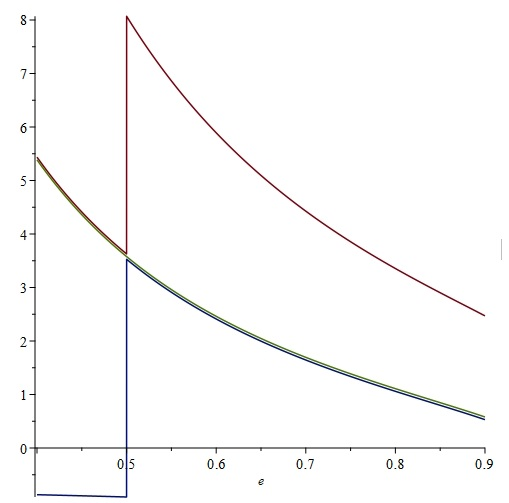
\includegraphics[scale=0.5]{imags/graphT.jpg}
				\end{center}
				\caption{$T_{ex}(e,l)$, красный --- по \ref{eq:TexLessHalf}, синий --- по \ref{eq:TexGreatHalf}, зелёный --- правильныйб, $l=0.2$}
				\label{graph:Tex}
			\end{figure}
			
			при маленьких $e$ верно, что
			\begin{equation}
				T_{ex}(e,l) = \cfrac{\pi}{2e^{3/2}} - 
				z + \cfrac{z^3}{6}-\cfrac{ez^5}{10} +...+ (-1)^k\cfrac{e^{k}z^{2k+3}}{(4k+6)}
				+...
			\end{equation}
			где
			\begin{equation}
				z = \cfrac{2\sqrt{1-e-l^2}}{1-2e}
			\end{equation}
			
			Замена $r = \cfrac{r_{-}+r_{+}}{2} - \cfrac{r_{+}-r_{-}}{2} \cos{\theta}$ приводит к уравнению:
			\begin{equation*}
				\dot{\theta}\cdot(1 - y\cdot\cos(\theta)) = \cfrac{2\sqrt{e}}{r_{-}+r_{+}} = 2e^{3/2}
			\end{equation*}
				где 
			\begin{equation*}
				y = \cfrac{r_{+}-r_{-}}{r_{-}+r_{+}} = \sqrt{1 - 4el^2}
			\end{equation*}
			тогда 
			\begin{equation*}
				\theta - y \sin{\theta} - (\theta_{-} - y\sin{\theta_{-}}) = 2e^{3/2}(t-t_{-})
			\end{equation*}
			
			если $G(y,z) $ --- обратная функция $\theta \rightarrow \theta - y \sin{\theta}$, тогда
			\begin{equation*}
				\theta = G(y,2e^{3/2}(t-t_{-}) + (\theta_{-} - y\sin{\theta_{-}})) 
			\end{equation*}
			при использовании временного параметра $\tau = t/T_{ex}(e,l)$, получаем
			\begin{equation*}
				\theta = G\left(y,\pi \cdot \left(\tau \cfrac{T_{ex}(e,l)}{T(e)} +
				\cfrac{T_{in}(e,l)}{T(e)}
				\right) \right) 
			\end{equation*}
			где $T_{in}$ --- внутренняя часть времени траектории, $T_{in} + T_{ex} = T(e) = \cfrac{\pi}{2e^{3/2}}$
			\begin{eqnarray*}
				\theta = G(y,\pi (1 -(1 - \tau)z ) ) \\
				z = \cfrac{T_{ex}(e,l)}{T(e)}
			\end{eqnarray*}
			\item Решение внутри
			
			Если $r_{max} < 1$, то всё тривиально, однако если $r_{max} > 1$, траектория гибридная. Во внутренней части её время является разрывной фенкцией параметров $e, l$. 
			Однако непрерывной является фунция $T_{\theta} = T_{in}/\theta_1$, где $\theta_1$ --- угол, соответствующий $r = 1$ в \ref{eq:tr_in_func}. $\theta_1$ тоже разрывен, но он равен
			\begin{equation}
				\cos{\theta_1} = -\cfrac{2-u_0-u_1}{u_1-u_0} = 
				-\cfrac{(2-u_0-u_1))}{\sqrt{(u_1-u_0)^2}} 
			\end{equation}
			И числитель и подкоренное значение знаменателя этой дроби является непрерывными по параметрам.
		\end{itemize}
	\end{enumerate}
	
	В интерполяции внутреннего времени есть дин нюанс: он разрывно зависит от $e$ и $l$.
	Продемонстрировать это можно тем, что при $e \rightarrow 1/2-0$ $\theta_1 \rightarrow \pi$, а когда  $l \rightarrow l_{max}$ --- $\theta_1 \rightarrow 0$. Тогда непрерывной будет величина 
	\begin{equation}
		T_{\theta in} = \cfrac{T_{in}}{\theta_1}
	\end{equation}
	
	Далее: при интерполяции времени по сетке $el$, озможно, что каждый бин придется разбить на более маленькие части для более точной интерполяции времени. Для этого квадратный бин можно разделить на части (сделаем это по переменным $e$ и $\xi = \sqrt{1-l^2/l_m^2}$)
	
	Итак, Алгоритм для интерполяции внутреннего преиода:
	\begin{itemize}
		\item Интерполяция $u_1^2-u_0^2$ и $u_0^2+u_1^2$
		\item можно интерполировать переменныые $r_1^2-r_0^2$ и $r_1^2+r_0^2$
		\item Получение $r_0$ и $r_1$
		\item Нахождение $\theta$
		\item Интерполяция $T_{\theta in}$ 
		\item Вычисление $T_{in}$
	\end{itemize}
	
	Вообще можно интерполировать ещё одну величину, равную
	\begin{equation}
		\cfrac{du_{e pm}}{\sqrt{1 - l^2}} = \cfrac{u_{pm} - u_l(e)}{\sqrt{1 - l^2}}  \rightarrow  ( l = L/L_{max}(e),  l \rightarrow 1)  \rightarrow  \pm \cfrac{L_{max}}{\sqrt{-1/2F''(u_e)}}
		\label{eq:duepm}
	\end{equation}
	Единственная проблема будет тогда, когда есть большое расхождение межде двумя радиусами, т.е. когда $l^2 \rightarrow 0$, поэтому такую интерполяцию нежелательно проводить при малых $l$.
	Предлагается использовать эту интерполяцию при условии, что в бине $l_{max} > 0.8$, иначе использовать простую интерполяцию $u_p$ и $u_m$
	
	Но и тут есть проблема, возникающая при $L^2 \approx 1-e$. Разложим $F(u)$ вблизи $u = 1$.
	 \begin{equation}
		F(u) = 1 + \frac{1}{2} (u-1) + \frac{F_2}{2}(u-1)^2
	 	]\label{eq:Fu_more_1}
	 \end{equation}
	 Решая $F(u) - eu - l^2 = 0$, получим:
	\begin{equation}
	 	u_{1,0} = 1 + q_e \pm \sqrt{q_e^2 + 2y}
	 	\label{eq:u01_near1}
	\end{equation}
	где
	\begin{eqnarray*}
		q_e = \cfrac{1-2e}{-2F_2}\\
		L^2 = (1-e) + F_2z
	\end{eqnarray*}
	
	Проблемная область поиска $\theta_1$ та, где $u_1 \rightarrow 1$, тогда $u_1 = 1 + \delta_1$. Когда $u_0$ отлично от $1$, можно использовать приближение:
	\begin{equation*}
		\cos {\theta_1} = -\cfrac{1-u_0-\delta_1}{1-u_0+\delta_1} = -\cfrac{1-x}{1+x} \rightrightarrows \theta_1 =  \pi - \arcsin {\cfrac{2\sqrt{x}}{1+x} } (x < 1), \arcsin {\cfrac{2\sqrt{x}}{1+x} } (x > 1)
	\end{equation*} 
	где $x = \delta_1/(1-u_0)$
	
	В случае, если ещё и $u_0 \rightarrow 1$ т.е. $u_0 = 1 - \delta_0$
	\begin{equation*}
		\cos {\theta_1} = -\cfrac{1-u_0-\delta_1}{1-u_0+\delta_1} = 
		-\cfrac{\delta_0-\delta_1}{\delta_0+\delta_1}
		\approx \cfrac{q_e}{\sqrt{q_e^2 + 2z}}
	\end{equation*}
	Если $\cos {\theta_1}$ разделить на эту дробь, то результат можно уже интерполировать.
	Также можно интерполировать 
	\begin{equation*}
		du2q = \left(\cfrac{u_1-u_0}{\sqrt{q^2+2z}}\right)^2 = \cfrac{(r_1-r_0)^2(r_1+r_0)^2}{q2z}
	\end{equation*}
	\begin{equation*}
		suq = \cfrac{u_1+u_0 - 2}{q}
	\end{equation*}
	
	При $e < 1/2$, $\delta_1$ известно, поэтому будем интерполировать величину
	\begin{equation*}
		\cfrac{\delta_0}{\sqrt{q_e^2+2z} - q_e} = 
		\delta_0\cdot\cfrac{q_e+\sqrt{q_e^2+2z}}{2z}
	\end{equation*}
	
	При $e > 1/2$, Находится величина $\delta_1$. С помощтю интерполяции.
	\begin{equation*}
		\cfrac{\delta_1}{\sqrt{q_e^2+2z} + q_e} = 
		\delta_1\cdot\cfrac{\sqrt{q_e^2+2z }- q_e}{2z}
	\end{equation*}
	
	Тут хотелось бы иметь гарантии, что $q_e^2 + 2z > 0$. Посмотрим, что тут у нас. Итак, это подкоренное выражение пропорционально величине $L_m'^2(e) - L^2$ для разложения функции $F(u)$ в \ref{eq:Fu_more_1}, где $L_m'^2(e)$ --- квадрат максимального момента. Нам надо, чтобы $L_m'^2(e) > L_m^2(e)$ Мы знаем, что
	\begin{equation*}
		 L_m^2(e) = F(u_e) - u_e \cdot e
	\end{equation*}
	при условии что 
	\begin{equation*}
		F'(u_e) - e = 0
	\end{equation*}
	в таком случае
	\begin{equation*}
		\cfrac{du_e}{de} = \cfrac{1}{F''}
	\end{equation*}
	а
	\begin{equation*}
		\cfrac{dL_m^2(e)}{de} = (F'(u_e) - e) \cfrac{du_e}{de} - u_e = -u_e
	\end{equation*}
	Как мы узнаем, $-F''$ --- убывающая положительная функция при $\rho'(r) < 0$. Поэтому для реального потенциала $du_e/de > du_e'/de$ поэтому $u_e > u_e'$ поэтому $dL_m^2(e)/de < dL_m'^2(e)/de$. 
	Но на всякий случай лучше заменить $\sqrt{q_e^2+2z}$, что равно $\sqrt{\cfrac{2}{-F_2}(L_e'^2-L^2)}$ на $\sqrt{\cfrac{2}{-F_2}(L_m^2-L^2)}$ при $e > 1/2$
	
	В зависимости от точки $E$ и $l$, нужно использовать разные способы интерполяции $u_0$ и $u_1$
	\begin{figure}[!h]
		\begin{center}
			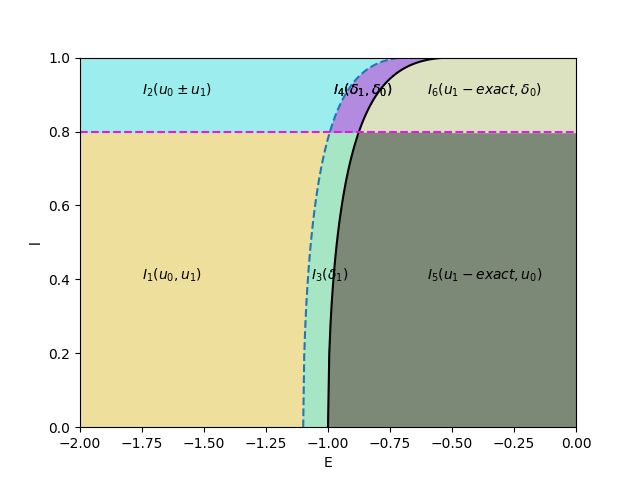
\includegraphics[scale=0.9]{imags/diagramm1.png}
		\end{center}
		\caption{Зоны на плоскости E-L}
		\label{diagramm1:Tex}
	\end{figure}
	
	Всего есть 6 случаев, они определяются переменной $l_u = L/L_m(e)$ и $z$: когда $l_u$ близко к $1$ или нет, когда $z$ положительный (справа)/ отрицательный(слева)
	\begin{itemize}
		\item Случай $l_u$ не близко к $1$: тогда $u_0$ можно интерполировать по $e,l$, и не боятся корневой нерегулярности, для $u_1$ существуют различные варианты:
		\begin{itemize}
			\item Область 1, 3, когда $u_1$ определяется так же как и $u_0$. Но менее $1$. 
			При этом $\theta_{max} = \pi$
			\item Область 5: $u_1$ определяется точно по формуле (\ref{eq:u01_near1})
		\end{itemize}
		\item Случай $l_u$ близко к $1$:
		\begin{itemize}
			\item В области 2,4 лучше интерполировать величину $u_1 + u_0$, которые непрерывны по $e$, $l$ и малую величину (\ref{eq:duepm}). Помним: $\theta_{max} = \pi$, $u_1<1$ 
			\item В области 6 $u_1$ определяется точно. Но нам нужно знать точно $\delta_0$. Для этого используется интерполяция по величине 
			\begin{equation*}
				\cfrac{\delta_0}{\sqrt{q_e^2+2z} - q_e} = 
				\delta_0\cdot\cfrac{q_e+\sqrt{q_e^2+2z}}{2z}
			\end{equation*}
		\end{itemize}
	\end{itemize}
	
	В области 1,3,5 нужно уточнить поведение при малых $l_u$. Для поиска $u_0$, $u_1$ мы решаем уравнение 
	\begin{equation*}
		F(u) - eu- L^2= 0 = u(\phi(u)-e) - L_m^2(e)l_u^2
	\end{equation*}
	при $e \rightarrow e_0$ $\phi(u)-e \approx e_0-e - C_0 u /2$
	тогда 
	\begin{equation*}
		u_0 \approx \cfrac{L_m^2(e)l_u^2}{e_0-e}
	\end{equation*}
	Это означает, что при больших $e_0-e$ мы можем интеорполировать величину $u_0/l_u^2$.
	Однако проблема возникает при малых $e_0-e$
	Тут мы воспользуемся разложением
	\begin{equation}
		F(u) \approx e_0 u + F''(0)/2 u^2 = 
		e_0 u - \frac{C_0}{2} u^2
		\label{eq:F_near_0}
	\end{equation}
	тогда (обозначим $e_0-e$ как $de$)
	\begin{equation}
	u_{0/1} \approx \cfrac{de \pm \sqrt{de^2-2C_0 L^2} }{C_0} =
	\cfrac{de \pm \sqrt{de^2-2C_0 L_m^2(e)\cdot l_u^2} }{C_0}
	\end{equation}
	
	При $de \rightarrow 0$ $L_m^2(e) \rightarrow \frac{de^2}{2C_0}$
	\begin{equation}
		u_{0/1} \approx de\cfrac{1 \pm \sqrt{1-l_u^2} }{C_0}
	\end{equation}
	тогда при малых $l_u$ $u_1$ можно просто интерполировать по $e,l$, а $u_0$ нужно находить из интерполяции величины
	\begin{equation}
		u_{0l} = \cfrac{u_0}{l_u^2} \rightarrow (l_u \rightarrow 0) \rightarrow 
		\cfrac{L_m^2(e)}{de} \approx (de \rightarrow 0) \approx \cfrac{de}{2 C_0}
		\label{eq:u_0l_interpol}
	\end{equation}
	Однако при малых $de$, интерполяция может происходить на всём интервале $l_u = 0..1$. тогда \ref{eq:u_0l_interpol} плохо работает. В этом случае можно интерполировать величину
	\begin{equation}
		u_{0s} = \cfrac{u_{0/1}}{1 - \sqrt{1-l_u^2}} =  \cfrac{u_{0/1}}{l_u^2} (1 + \sqrt{1-l_u^2})  \rightarrow (l_u \rightarrow 0) \rightarrow 
		2\cfrac{L_m^2(e)}{de} \approx (de \rightarrow 0) \approx \cfrac{de}{C_0}
		\label{eq:u_0l_soph_interpol}
	\end{equation}
	
		
	\subsubsection{Потенциал.}
	Свяжем величины: безразмерный потенциал $\varphi(r)$, безразмерный радиус $r$, безразмерная масса $M(r)$ (такая, что $M(1) = 1$), безразмерная плотность $\rho(r)$.
	\begin{eqnarray*}
		\cfrac{M(r)}{r^2} = -\varphi'(r) \\
		3\rho(r) = \cfrac{M'(r)}{r^2}
	\end{eqnarray*}
	В дальнейшем нам понадобится непрерывная функция 
	\begin{equation}
		Q(r) = \cfrac{M(r)}{r^3}
	\end{equation}	
	Для нахождения $Q(r)$ будем делить на $r^3$ $M(r)$, которая определяется квадратурой Гаусса.
	\begin{equation}
		Q(r+h) = \cfrac{Q(r)r^3 + I_G[r \rightarrow  3\rho(r)r^2](r,r+h)}{(r+h)^3}
	\end{equation}
	
	После численного интегрирования мы получим $Q(1) \ne 1$, поэтому необходимо будет разделить $Q(r)$ и $\rho(r)$ на $Q(1)$.
	
	Для получения потенциала останется лишь проинтегрировать непрерывную функцию $rQ(r)$ с помощью квадратур Гаусса.
	
	\subsubsection{Вычисление функция $S(u)$}
	Мы хотим вычислить функцию 
	\begin{equation}
		S(u) = \cfrac{u\varphi(u) -eu-l^2}{(u-u_{-})(u_{+}-u)}
	\end{equation}
	Положим $F(u) = u\varphi(u)$.
	Тогда 
	\begin{equation}
		S(u) = \cfrac{1}{u_{+}-u_{-}}\cdot 
		\left(\cfrac{F(u)-F(u_{-})}{u-u_{-}} - \cfrac{F(u_{+})-F(u)}{u_{+}-u}\right)
	\end{equation}
	Эта функция является непрерывной и определенной, однако при близких значениях $u_{+}, u_{-}, u$ необходимо вычисление с помощью производных.
	Возможные случаи:
	\begin{itemize}
		\item $u_{+}$ близко к $u_{-}$. В этом случае получаем, что 
		\begin{equation}
			S(u) = -\cfrac{1}{2}F''\left(\cfrac{u_{+} + u_{-} + u}{3}\right)
		\end{equation}
		
		\item $u$ близко к $u_{-}$, но далеко от $u_{+}$ (либо наоборот). Тогда через производные оцениваем только первую разность.
		\begin{equation}
			S(u) = \cfrac{1}{u_{+}-u_{-}}\cdot 
			\left(F'\left(\cfrac{u+u_{-}}{2}\right) - \cfrac{F(u_{+})-F(u)}{u_{+}-u}\right)
		\end{equation}
		Далее --- очевидные формулы без текста.
		\begin{eqnarray}
			\deriv{}{u} = \cfrac{1}{2r}\deriv{}{r}\\
			F'(u) = \cfrac{1}{2r}\deriv{}{r}(r^2\varphi(r)) = 
			\varphi(r) + \cfrac{r\varphi'(r)}{2} = \varphi(r) -\cfrac{r^2}{2} Q(r) \\
			F_2 = F''(u) = \cfrac{1}{4}
			\left( \varphi''(r) + 3\cfrac{\varphi'(r)}{r}\right) = -\cfrac{1}{4}\left(3\rho(r) + Q(r)\right)
		\end{eqnarray}
		Видно, что $F(u)$ --- выпуклая вниз и монотонная функция, поскольку $F''(u) < 0$, а $F'(\infty) = 0$ и производная убывает, то $F'(u) > 0$
		Также заметим, что
		\begin{equation*}
			\cfrac{dF_2}{dr} = -\frac{3}{4}\left(
			\rho'(r) + \cfrac{\rho(r)}{r} - \cfrac{\int_0^r{3\rho(r')r'^2dr'}}{r^4}
			\right) = 
			\frac{3}{4r}\left(
				\cfrac{\int_0^r{3(\rho(r')- \rho(r))r'^2dr'}}{r^3}
				- r\rho'(r)
			\right)
		\end{equation*}
		пожтому, если $\rho(r)$ --- убывающая функция (что довольно естественно), то $F''(u)$ --- возрастающая функция.
	\end{itemize}
	
	В случае если $u_p, u > 1$ (т.е. $e < 1/2$) Мы заменим функцию $F(u)$ на полином
	\begin{equation*}
		F(u) = 1 + \cfrac{u-1}{2}-\cfrac{(u-1)^2}{8}
	\end{equation*}
	Тогда максимальное значение $u_p$ на мнимой траектории равно
	\begin{equation*}
		u_p = -4e + 3 + 2\sqrt{4e^2 - 2l^2 - 6e + 3}
	\end{equation*}
	
	
	
	\subsubsection{Нахождение $l_m(e)$}
	\begin{itemize}
		\item при $e \le \frac{1}{2}$ $l_m^2(e) = 1-e$ --- определяется из условия пересечения траектории с телом
		\item если условием пересечения пренебречь, то $l_m^2(e) = \frac{1}{4e}$. 
		\item Когда $e > \frac{1}{2}$, необходимо находить $l_m(e)$ из \ref{eq:l_m_e}.
		Дифференцируя это выражение по $u$, получаем уравнение 
		\begin{equation*}
			F'(u) - e = 0
		\end{equation*}
		Как мы уже знаем, $F''(u) > 0$. Это заначит, что корень уравнения можно найти методом бинарного поиска, так как $F'(u)$ убывает.
	
	\end{itemize}
	Найдя близжайшие точки $r_1, r_2$ на узлах сетки $r_i$, мы уточним решение, приблизив функцию $F'(u(r))$ линейно. Тогда 
	\begin{equation*}
		r_m = \cfrac{r_2 F'(r_1) - r_1 F'(r_2)}{F'(r_1)-F'(r_2)}
	\end{equation*}
	
	Также можно дополнительно уточнить, сделав шаг методом Ньютона
	\begin{equation*}
		r'_m = r_m - \cfrac{F'(r_m)}{F''(r_m)}
	\end{equation*}
	
	Кастати, итерацию ньютона можно модифицировать для случая обнуления первой производной.
	\begin{equation*}
		x' = x - \cfrac{2f(x)}
		{f'(x) +sgn(f'(x))\sqrt{f'(x)^2 - 2f(x)f''(x)} }
	\end{equation*}
		
	\subsubsection{Нахождение концов траектории.}
	Концы траектории определяются соотношением
	\begin{equation*}
		\Phi(u) = F(u) - eu-l^2=0
	\end{equation*}
	Так как $\Phi'(u) = F'(u) - e$ --- функция, которая убывает, причем $\Phi'(u_m(e)) = 0$, то $\Phi(u)$ --- возрастает при $u < u_m(e)$ и убывает при $u > u_m(e)$.
	Таким образом, $\Phi(r)$ ведет себя так же как $\Phi(u)$, тогда для нахождения корней нужно лишь использовать метрд деления отрезка попола, а уточнить можно методом ньютона. 
	
	
	\subsubsection{Переход из фазовых объемов.}
	Задача номер 1 сводится к нахождению концентрации частиц в точке $r$, зная распределение частиц в плоскости $E-L$.
	
	Итак, фазовый объем предсавляется в виде
	\begin{equation}
		\label{eq:phase_volume_nd}
		d\Phi = r_{\odot}^3v_{esc}^3 \cdot 4\pi^{2} d\tau de dl^2
	\end{equation}
	А также в виде
	\begin{equation}
		d\Phi = r_{\odot}^3v_{esc}^3 \cdot d^3\vec{r}d^3\vec{v}
	\end{equation}
	
	Самое простое, что можно найти - это полная фазовая плотность
	
	\begin{equation*}
		\cfrac{dN}{d^r dv_r dv_{tau}} = 
		\cfrac{dn(r)}{dv_r dv_{tau}} = 
		4\pi v_{tau}\cfrac{dn(r)}{d^3v} = 
		v_{tau}\cfrac{dN}{\pi d\tau de dl^2} = 
		\cfrac{dN(e,l)}{2\pi r T(e,l) de dl}
	\end{equation*}
	
	Учтем также, что
	\begin{equation}
		\label{eq:velocity_dens}
		d^{3}\vec{v}  = 2\pi ded\sqrt{v^2-\frac{l^2}{r^2}} d\vec{n}.
	\end{equation}
	 
	 Причем, поскольку радиальная скорость $v_r$ и тангенциальная $v_{t}$ фиксированны, для $d\vec{n}$ остается только выбор направления для тангенциальной скорости ($\int{d\vec{n}} = 1$).
	 
	 Отсюда получаем, что
	 
	 \begin{equation}
	 	n(r) = \int{ \cfrac{dN}{2\pi T(e,l) de dl^2} de d\sqrt{v^2-\frac{l^2}{r^2}}}
	 \end{equation}
	 
	 \begin{enumerate}
	 	\item Предположение 1: равномерное распределение внутри бина по $dedl$:
	 	
	 	В этом случае 
	 	\begin{equation}
	 		f_1(e,l) = \cfrac{dN}{de dl}
	 	\end{equation}
	 	
	 	И тогда получим
	 	\begin{equation}
	 		\label{eq:n_r}
	 		n(r) = \int{ \cfrac{1}{r} \cfrac{f_1(e,l) }{4\pi T(e,l)} de \, d\asin{\cfrac{l}{rv}} }
	 	\end{equation}
	 	
	 	Если нужно генерировать распределение, то $L$ --- генерируется равномерно, т.е.
	 	\begin{eqnarray}
			L = (l_0 + (l_1-l_0)\xi)L_{max}(e) 		
	 	\end{eqnarray}
	 	где $l_i = L/L_{max}{e}$ --- приведенный момент импульса, а $\xi$ --- случайная величина в интервале $[0,1]$.
	 	
	 	А энергия генеируется НЕРАВНОМЕРНО:
	 	\begin{eqnarray}
	 		e = e_0 + (e_1-e_0)\cdot u \\
	 		u = \cfrac{2\xi}{(1-b)+\sqrt{(1-b)^2+4b\xi}} \\
	 		b = \cfrac{L_{max}(e_0)-L_{max}(e_0)}{L_{max}(e_0)+L_{max}(e_0)}
	 	\end{eqnarray}
	 	
	 	
	 	
	 	\item Предположение 2: равномерное распределение внутри бина по $dedl^2$:
	 	
	 	В этом случае 
	 	\begin{equation}
	 		f_2(e,l) = \cfrac{dN}{de dl^2}
	 	\end{equation}
	 	
	 	И тогда получим
	 	\begin{equation}
	 		n(r) = \int{\cfrac{f_2(e,l) }{2\pi T(e,l)} de \, d\sqrt{v^2-\frac{l^2}{r^2}} }
	 	\end{equation}
	 	
	 	Генерация $L$:
	 	\begin{eqnarray}
	 		L = \sqrt{l^2_0 + (l^2_1-l^2_0)\xi}L_{max}(e) 		
	 	\end{eqnarray}
	 	\begin{eqnarray}
	 		e = e_0 + (e_1-e_0)\cdot u \\
	 		u = \cfrac{\xi(3 + b^2)}{(1-b)^2+(1-b)\sqrt[3]{(1-b)^3+2\xi b(3 + b^2)} + \sqrt[3]{\cdots}^2} \\
	 		b = \cfrac{L_{max}(e_0)-L_{max}(e_0)}{L_{max}(e_0)+L_{max}(e_0)}
	 	\end{eqnarray}
	 	
	 		
	 	Интеграл легче всего взять методом монте-карло (это не очень затратно и просто реализуется).
	 	
	 	При этом важно учитывать пределы интегрирования не только исходя из размеров бина $[e_0,e_1],[\overline{l}_0,\overline{l}_1]$ но и из области определения подинтегральных фунций: $e<\varphi(r), l<rv = \sqrt{r^2(\varphi(r)-e)}$.
	 	
	 	Чтобы упростить вычисление, $e$ мы будем генерировать также, с тем же весом, однако $l$ необходимо получать в новых пределах, для этого меру бина в каждой МК итерации нужно умножать на 
	 	\begin{equation*}
	 		m(e) = \cfrac{l_{max}'-l_{min}}
	 		{l_{max}-l_{min}}
	 	\end{equation*}
	 	где 
	 	\begin{equation*}
	 		l_{max}' = \sqrt{r^2(\varphi(r)-e)}
	 	\end{equation*}
	 	
	 	Ещё одно замечание касаемо этого ограничения: пределы интегрирования $e$ тоже необходимо скорректировать.
	 	
	 	\begin{eqnarray}
	 		L_{min/max}(e) = L_0 + \cfrac{e-e_0}{e_1-e_0} \cdot (L_1-L_0)
	 		\\
	 		L^2_{restrict}(e) = r^2(\varphi(r)-e)	 		
	 	\end{eqnarray}
	 	
	 \end{enumerate}
	 
	 Вторая интересующая нас величина --- скорость аннигиляции
	 
	 \begin{equation}
	 	\label{eq:ann_st}
	 	\int{d^3\vec{r} d^3\vec{v}  d^3\vec{v_1} 
	 		f(\vec{r},\vec{v})f_1(\vec{r},\vec{v_1}) \sigma_{ann} 
	 		|\vec{v}-\vec{v}_1|} = \cfrac{\sigma_{a0}v_{a0}}{r_{\odot}^3} \int{dN_1 dn_2(r) \phi_{ann}(v) }.
	 \end{equation}
	 
	 где $\sigma_{a0}v_{a0}$ --- размерное сечение $*$ скорость взятое при произвольной скорости $v_{a0}$, а 
	 
	\begin{equation}
		\phi_{ann} = \cfrac{\sigma_{ann} |\vec{v}-\vec{v}_1| }{\sigma_{a0}  v_{a0}}.
	\end{equation}
	
	$dN_1$ --- дифференциал количества частиц сорта 1, $dn_2(r)$ --- дифференциал концентрации частиц сорта 2  (из \ref{eq:n_r})
	
	\begin{equation}
		dN_1 \approx \cfrac{dN_1}{T(e_1,l_1)de_1 dl_1^2} d\tau de_1 dl_1^2 \approx \cfrac{dN_1}{T(e_1,l_1)de_1 dl_1} d\tau de_1 dl_1 
	\end{equation}
	
	Величина $\phi_{ann}$ зависит от разности скоростей и равна $\phi_0 + \phi_2 v^2 +...$. При интегрировании можно вычислить эту величину для каждого члена ряда $v^i$ а потом просуммировать с весами $\phi_i$
	
	Вклад $v^2$ можно оптимизировать, так как если мы интегрируем по скоростям двух частиц, то скорости $\vec{v}_i$ и $-\vec{v}_i$ входят с одинаковым весом. Тогда можно сделать замену
	\begin{equation}
		v^2 = (\vec{v}_1-\vec{v}_2)^2 \rightarrow \frac{1}{2}\left(
			(\vec{v}_1-\vec{v}_2)^2 + 
			(\vec{v}_1+\vec{v}_2)^2
		\right) = \frac{1}{2}(v_1^2+v_2^2)
	\end{equation}
	
	\subsubsection{Проверки}
	1) Проверка захвата --- по статье. согласие есть
	
	2) Проверка Scatter --- Проверить полное сечение соударения для $\sigma = 1/v$
	
	3) Проверка концентрации: сохранение числа частиц $\sum_i{N_i} = \int{n(r)dV}$
	
	4) Проверка аннигилляции: при $\sigma v = 1$ аннигиляция равна $\int{n^2(r)dV}$.
	
	
	\subsubsection{Нормировка}
	
	
	\begin{itemize}
		\item Количество частиц:
		
		Полное число частиц в бине $i$ $N_{ri}$ должно равнятся
		\begin{equation*}
			N_{ri} = N_i \cdot N_{\odot}
		\end{equation*}
		где $N_{\odot} = n_{\chi,\infty}\cdot V_{\odot}$,  $N_i$ --- нормированное число частиц, участвующее в расчёте, $n_{\chi,\infty}$ --- концентрация Т.М. в гало, $V_{\odot}$ --- объём тела.
		\item Характерное время (частота соударений)
		
		В качестве единицы, обратного времени свободного пробега будем обозначать величину
		\begin{equation*}
			\cfrac{1}{T_{\chi p}} = 
			\sigma_{\xi p} \overline{n}_p V_{esc}
		\end{equation*}
		где $\overline{n}_p$ --- средняя концентрация протонов, $V_{esc}$ --- вторая космическая скорость для объекта, $\sigma_{\xi p}$ --- сечение нормировки (сечение рассеяния Т.М. на протоне/нуклоне при некой фиксиоровванной выбранной скорости $v = |\vec{v}_{\chi} - \vec{v}_p|$. Важно, что при более сложных потенциалах или в неупругом случае) 
		
		Естественно, мы обезразмерим реальное время: $t_r = T_{\chi p} t$
		\item Скорость захвата
		
		Полная скорость захвата в $i$том бине равна
		\begin{equation*}
			C_i = c_i \cfrac{N_{\odot}}{T_{\chi p}} 
		\end{equation*}
		
		Тогда темп захвата определяется из
		\begin{equation*}
			\cfrac{dN_{ri}^{capt}}{dt_r} = C_i \Leftrightarrow \cfrac{d N_{i}^{capt}}{dt} = c_i
		\end{equation*}
		
		Формуля для неупругого сечения (в системе центра масс):
		\begin{equation*}
			\cfrac{d\sigma}{d\Omega} = \cfrac{|\mathcal{M}|^2}{64\pi^2(E_1+E_2)^2}\cdot \cfrac{|\vec{v}_1'-\vec{v}_2'|}{|\vec{v}_1-\vec{v}_2|}
		\end{equation*}
		
		Под ядерным форм фактором понимается величина
		\begin{equation*}
			F(q,v) = \cfrac{|\mathcal{M}|^2}{|\mathcal{M}_0|^2} \cdot \cfrac{(m_{\chi}+m_{p})^2}{(m_{\chi}+m_{N})^2}
		\end{equation*}
		где $m_{N}$ --- масса ядра, $m_{p}$ --- массса одного нуклона, по которому идет нормировка.
		
		Под $\sigma_{\xi p}$ подразумевается величина
		\begin{equation*}
			\sigma_{\xi p} = \int{\cfrac{ |\mathcal{M}_0|^2  }{64\pi^2 (E_p+E_{\chi})^2} d\Omega}
		\end{equation*}
		
		Тогда, используя безразмерные параметры, получаем:
		\begin{equation*}
			c_i = \int{ dr^3 \int{d^3\vec{v}_{\chi}\int{ \widetilde{f}(\vec{v}_{\chi}) 
				\widetilde{n}_N(r)  \cdot |\vec{v}_{\chi}'-\vec{v}_{N}'| F(q,v) d\vec{n}'_{CM} }}} 
		\end{equation*}
		
		где функция распределения ТМ равна $n_{\chi,\infty} \widetilde{f}(\vec{v}_{\chi})$, $d\vec{n}'_{CM}$ --- элемент выходного фазового объема (направление выходной скорости в системе Ц.М.), полный интеграл которого равен 1 ($\int {d\vec{n}'_{CM} } = 1$)
		\begin{equation*}
			d\vec{n}'_{CM} = \cfrac{d\cos{\theta'} d \varphi' }{4\pi}
		\end{equation*}
		
		Начальная скорость: 
		\begin{equation*}
			d^3\vec{v}_{\chi} \widetilde{f}(\vec{v}_{\chi}) = 2\pi v dv^2 f_e(v^2) = 2\pi v du^2 f_e(u^2)  
		\end{equation*}
		где $v^2 = v^2_{esc}(r) + u^2$, $v_{esc}(r)$ --- скорость вылета в точке $r$, $u$ --- скорость на бесконечности $f_e(u^2)$ --- эффективная плотность на бесконечности с учётом скорости движения небесного тела относительно гало $u_0$ ($\vec{u} = \vec{u}_0 + \vec{w}$) где $\vec{w}$ --- скорость в гало. 
		\begin{equation*}
			f_e(u^2) = \int_{-1}^1 {f(u^2+u^2_0 + 2 u u_0 x) \cfrac{dx}{2}}
		\end{equation*}
		
		\item Темп рассеяния
		
		Обезразмеренная матрица рассеяния (тоже на $T_{\chi p}$) $s_{ij}$ определяется из 
		темпа расеяния частиц (тоже обезразмеренного):
		\begin{equation*}
		\cfrac{d N_{i}^{scat}}{dt} = s_{ij} N_j
		\end{equation*}
		
		\item Безразмерная концентрация ТМ:
		
		\begin{equation*}
			\tilde{n}_{\chi}(r) = \sum_i{\int{\cfrac{4\pi}{3} \cfrac{1}{2\pi T(e,l)} \cfrac{dN_i}{dedl^2} de d\sqrt{v^2-\frac{l^2}{r^2}} }}
		\end{equation*}
		 В таком случае
		 \begin{equation*}
		 	\int{\tilde{n}_{\chi}(r) 3r^2dr} = \sum{N_i} = \sum{\cfrac{N_{ri}}{V n_{\chi \infty}}}
		 \end{equation*}
		 Такой выбор размерности связан с тем, что $V \cdot 3r^2dr = dV$ и тогда
		 \begin{equation*}
		 	\int{\tilde{n}_{\chi}(r) n_{\chi \infty} dV} = \sum{N_{ri}} = \text{Полное число частиц}
		 \end{equation*}
		\item Аннигиляция:
		Мы хотим чтобы
		\begin{equation}
			\cfrac{d N_{i}^{ann}}{dt} = \gamma_p a^{p}_{ij} N_j N_i
		\end{equation}
		где 
		\begin{equation*}
			\gamma_p = T_{\chi p} \cdot n_{\chi \infty} \langle\sigma_{ann} v\rangle_{v = v_{esc}}
		\end{equation*}
		отношение темпа аннигиляции к темпу рассеяния. Важно: величина сечения аннигиляции $\langle\sigma_{ann} v\rangle$ берётся при скорости $v = v_{esc}$ (для аннигиляции сечение которой ведёт себя как $\langle\sigma_{ann} v\rangle = const\cdot v^2$)
		
		\begin{equation*}
			a_{ij}^p = \int{\phi_{ann} 3r^2dr\left(\cfrac{4\pi}{3}\right)^2 \left( \cfrac{1}{2\pi T(e_1,l_1)} \cfrac{1}{de_1dl_1^2} de_1 d\sqrt{v_1^2-\frac{l_1^2}{r^2}} \right) \left( \cfrac{1}{2\pi T(e_2,l_2)} \cfrac{1}{de_2dl_2^2} de_2 d\sqrt{v_2^2-\frac{l_2^2}{r^2}} \right)}
		\end{equation*}
		Из этого поределения следует:
		\begin{equation*}
			a_{ij}^p N_i N_j = \int{3r^2dr \tilde{n}^2_{\chi}(r) \phi_{ann}}
		\end{equation*}
		Полная скорость аннигиляции равна
		\begin{equation*}
			\cfrac{dN^{ann}_{ri}}{dt_r} = \gamma_p a_{ij}^p N_i N_j \cdot \cfrac{N^2_{\odot}}{T_{\chi p}}
		\end{equation*}
		
	\end{itemize}
 
	
	
\end{document}